\chapter*[Introdução]{Introdução}
\addcontentsline{toc}{chapter}{Introdução}

Este capítulo irá apresentar a contextualização deste trabalho, o tema proposto, o problema que se tentou resolver, os objetivos almejados e como o trabalho está organizado.

Desde a sua concepção, \textit{sites} de redes sociais têm atraído milhões de usuários, muitos dos quais têm integrado esses \textit{sites} em suas rotinas diárias. Existem centenas de redes sociais com diversas capacidades tecnológicas suportando uma ampla gama de interesses e práticas. Os principais recursos tecnológicos envolvidos são bem consistentes e semelhantes, porém as culturas que estão impregnadas podem variar bastante. Alguns \textit{sites} tendem a atender diversos tipos de pessoas com interesses variados, outros se voltam a grupos mais específicos, que se comunicam em uma linguagem comum possuem outros interesses \cite{Boyd:Ellison:2007}.

Nos últimos tempos, sistemas que promovem a interação de pessoas, o compartilhamento de informações e a formação de grupos como as redes sociais, deixaram de ser uma tendência, e se estabeleceram de maneira irreversível. Tal fato tem atraído cada vez mais pessoas para o uso dessas tecnologias, mudando a forma de interação e comunicação entre os indivíduos \cite{Santana:Melo-Solarte:Neris:Miranda:Baranauskas:2009}.

O aumento do número de usuários de redes sociais dá-se principalmente pela facilidade de acesso das pessoas a aparelhos que permitem se conectar a internet a qualquer hora e em qualquer lugar, como é o caso dos smartphones. Como pode ser visualizado na Figura \ref{social_network_brazil} o Brasil, até o ano de 2017, faz-se uma projeção de que cerca de 110 milhões de pessoas utilizem as redes sociais, o que representa mais de 89\% dos usuários com acesso à internet \cite{eMarketer:2013}.

\newpage

\begin{figure}[!h]
	\centering
	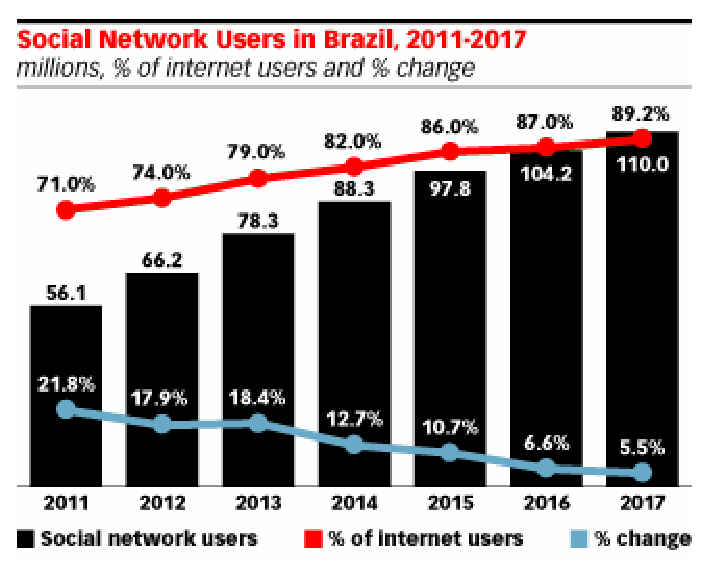
\includegraphics[scale=0.8]{figuras/capitulo1/social_network_brazil.eps}
	\caption[Uso de redes sociais no Brasil]{Uso de redes sociais no Brasil \cite{eMarketer:2013}}
	\label{social_network_brazil}
\end{figure}

Visando colaborar com o contexto de redes sociais, busca-se apresentar uma ferramenta que auxilie desenvolvedores a criar sistemas desse tipo, oferecendo recursos que são comuns à maioria das aplicações sociais. Mais precisamente, esse trabalho propõe-se a desenvolver um \textit{framework} que ofereça esses recursos para o desenvolvedor. Nas próximas seções, essa ideia será contextualizada e justificada.

\section*{Contextualização}
\addcontentsline{toc}{section}{Contextualização}

Uma rede social virtual é uma comunidade \textit{online} que representa um conjunto de participantes (pessoas, organizações ou outras entidades), unindo ideias e recursos em torno de relacionamentos, valores e interesses compartilhados \cite{Marteleto:2001}.

Diversos sistemas conhecidos parecem estruturados como uma rede. Para a Biologia, há o interesse em saber quem se alimenta de quem, quando se estuda a cadeia alimentar. O cérebro faz ligações entre neurônios; as sinapses, para que a pessoa lembre ou resolva algum problema ou questão. A Internet é uma rede na qual as pessoas se conectam e se comunicam. As doenças, por exemplo, podem se propagar de uma pessoa para outras, deflagrando uma epidemia \cite{Goular:2014}.

Assim, a análise da relação entre os nós e da estrutura formada pela rede fornece informações a respeito de diversos fenômenos e situações: como o cérebro funciona, como a doença se propaga, como as pessoas se comunicam e trocam informações, isto é, as relações ou interações influenciam a própria rede \cite{Goular:2014}.

A relação entre os nós da rede tem várias denominações apresentadas em trabalhos científicos: vínculo, ligação, arco, interação, conexão e/ou relação. Os nós da rede, também chamados de atores, estão ligados por essas relações. Por exemplo, os atores podem se classificar como amigos, quem troca informação com quem, quem confia em quem. A relação pode indicar que os atores fazem parte de um clube, de uma associação, trabalham no mesmo departamento ou que mantêm transações comerciais, trocam mensagens, trabalham em equipe ou cooperam entre si para algum tipo de trabalho. Os atores podem ser pessoas ou empresas que estão relacionadas por alguma atividade, além de grupos, localidades, cidades, regiões, entre outros \cite{Hanneman:Riddle:2005}.

John Scott, em seu livro \cite{Scott:Carrington:2011}, diz que redes sociais são formadas por dois tipos principais de dados: dados de atributos e dados de relacionamentos. Diz-se que os dados de atributos são as opiniões e os comportamentos dos agentes demonstrados dentro da rede. Portanto, são qualidades e características que pertencem a eles como indivíduos. Esses dados podem ser quantificados e analisados. Os dados de relacionamentos dizem respeito aos contatos, laços e conexões. Esses dados não são dados de um agente, e sim, de um conjunto de agentes conectados que formam um sistema de relacionamentos. É possível também quantificar e analisar esses tipos de dados, podendo encontrar padrões de relacionamentos em grupos.

Para abstrair o contexto do mundo real para o mundo computacional deve-se utilizar um software para prover mecanismos de análise para melhor planejar e manter a rede de uma organização. Tendo como foco o produto de software e baseando-se nas plataformas tecnológicas, deve-se levar em conta a reutilização de software. Essa necessidade é evidenciada, pois uma empresa geralmente deixa de construir um produto de software isolado, e busca parcerias para construir suas soluções \cite{Lima:2015}.

A reutilização de software é o processo de criar sistemas de software a partir de um software já existente, ao invés de criar a partir do zero \cite{Krueger:1992}. A meta da reutilização de software é reciclar o \textit{design}, código e outros componentes de um software e, assim, reduzir o custo, o tempo e melhorar a qualidade do produto \cite{Keswani:Joshi:Jatain:2014}.

Mesmo com todos os benefícios mencionados anteriormente, ao lidar com reutilização de software, deve-se planejar e conhecer bem quais são os objetivos esperados a partir dessa prática, como afirmam os autores Keswani, Joshi e Jatain, em sua publicação  \cite{Keswani:Joshi:Jatain:2014}, sobre reutilização de software: ``\textit{Para que um programa de reutilização de software confira o retorno apropriado, o mesmo deve ser sistematizado e planejado. Uma organização que implementa reutilização deve identificar os melhores métodos e estratégias para alcançar máxima produtividade}''.

\section*{Questão de Pesquisa}
\addcontentsline{toc}{section}{Questão de Pesquisa}

Esse trabalho tem como intuito responder com a seguinte questão: É possível oferecer um \textit{framework} que auxilie no desenvolvimento de redes sociais, disponibilizando recursos gerais de relacionamentos e específicos de definições de rotas e agenda, proporcionando ao desenvolvedor facilidade ao lidar com preocupações intrínsecas desse contexto?

\section*{Justificativa}
\addcontentsline{toc}{section}{Justificativa}

As redes sociais ultrapassaram o âmbito acadêmico/científico, conquistando espaço em outras esferas. É possível observar esse movimento na Internet, onde encontramos adeptos com objetivos específicos \cite{Tomae:Alcara:Chiara:2005}.

Nas últimas décadas, o trabalho pessoal em redes de conexões passou a ser percebido como um instrumento organizacional, apesar de o envolvimento das pessoas em redes fazer parte da história da humanidade há muito tempo \cite{Tomae:Alcara:Chiara:2005}.

Com tal crescimento e repercussão, torna-se pertinente a criação de um suporte que auxilie a produção de novas redes sociais digitais. Diante dessa questão, este trabalho propõe a criação de um \textit{framework} em atendimento a esse tópico, focando em redes mais específicas, as quais fazem uso de definições de rotas ou controle de relacionamento de agendas.

\section*{Objetivos}
\addcontentsline{toc}{section}{Objetivos}

Esse trabalho contém objetivos geral e específicos, conforme colocado nos subtópicos a seguir apresentados.

\subsection*{Objetivo Geral}
\addcontentsline{toc}{section}{Objetivo Geral}

Oferecer um \textit{framework} para ser utilizado no desenvolvimento de redes sociais, o qual disponibiliza recursos gerais de relacionamentos e específicos de definição de rotas e agenda, procurando auxiliar o desenvolvedor de software ao lidar com preocupações intrínsecas desse contexto.

\subsection*{Objetivos Específicos}
\addcontentsline{toc}{section}{Objetivos Específicos}

A partir do objetivo geral, pôde-se definir os objetivos específicos, os quais são:

\begin{enumerate}
	\item Definir uma arquitetura com base no uso de grafos, alinhada às boas práticas da Engenharia de Software, para representar os relacionamento entre as pessoas bem como as rotas percorridas por elas;
	\item Evoluir a arquitetura proposta, visando projetar algoritmos para compatibilizar agendas entre os interessados;
	\item Usar estruturas de dados e algoritmos específicos, visando desempenho e facilidades na manutenção evolutiva do software;
	\item Instanciar um produto de software - i.e. uma rede social específica - a partir do \textit{framework}, no intuito de coletar as primeiras impressões acerca do suporte desenvolvido como tema foco desse trabalho.
\end{enumerate}

\section*{Organização do documento}
\addcontentsline{toc}{section}{Organização do documento}

Este documento foi dividido em oito capítulos que são descritos brevemente à seguir:

\begin{enumerate}
	\item ~\nameref{chapter:Referencial_Teorico}: Levantamento bibliográfico de tópicos relevantes para alcançar o embasamento teórico necessário para a realização deste trabalho;
	\item ~\nameref{chapter:Suporte_Tecnologico}: Exposição das principais ferramentas e tecnologias que foram utilizadas no decorrer deste trabalho;
	\item ~\nameref{chapter:Metodologia}: Apresentação de como foi conduzido o trabalho, abordando modelos de desenvolvimento e modelos de pesquisa utilizados;
	\item ~\nameref{chapter:Proposta}: Apresentação completa do que este trabalho se propôs a fazer;
	\item ~\nameref{chapter:SocialFramework}: Apresentação do \textit{framework} desenvolvido durante deste trabalho;
	\item ~\nameref{chapter:Resultados}: Apresentação dos resultados obtidos durante todo o desenvolvimento do trabalho;
	\item ~\nameref{chapter:Conclusao}: Apresentação do que se pode concluir com ao término do trabalho.
\end{enumerate}
